\documentclass[aspectratio=169]{beamer}
\usepackage[utf8]{inputenc}
\usepackage[T1]{fontenc}
\usepackage[french]{babel}
\usepackage{tikz}
\usepackage{amsmath}

\usetikzlibrary{decorations.pathreplacing, fit, backgrounds, calc, shapes.geometric, arrows.meta, positioning, shadows.blur}
\tikzset{
  box/.style={
    rectangle, rounded corners, minimum width=4cm, minimum height=1.2cm,
    text centered, draw=black, fill=blue!20,
    drop shadow={shadow xshift=0.5ex,shadow yshift=-0.5ex,opacity=0.2}
  },
  service/.style={
    rectangle, rounded corners, minimum width=3.8cm, minimum height=1cm,
    text centered, draw=black, fill=green!25,
    drop shadow={shadow xshift=0.3ex,shadow yshift=-0.3ex,opacity=0.15}
  },
  departement/.style={
    rectangle, rounded corners, minimum width=5cm, minimum height=1.1cm,
    text centered, draw=black, fill=orange!30,
    drop shadow={shadow xshift=0.4ex,shadow yshift=-0.4ex,opacity=0.2}
  },
  conseil/.style={
    rectangle, rounded corners, minimum width=5.2cm, minimum height=1.1cm,
    text centered, draw=black, fill=red!30,
    drop shadow={shadow xshift=0.4ex,shadow yshift=-0.4ex,opacity=0.2}
  },
  arrow/.style={
    ->,>=Stealth, line width=0.4pt, color=gray!60
  }
}


\usetheme{Madrid}
\usecolortheme{default}

\title[Stage de recherche]{Optimisation d'un algorithme de calcul de bornes de latences pour accélérer la génération de preuves}
\author{Florian Delage}
\institute[NCPP]{La Prépa des INP\ --\ Nancy}
\date{\today}
\logo{
\includegraphics[height=1cm]{little_logo_prepa.png}}

\AtBeginSection{
  \begin{frame}
    \frametitle{Table des Matières}
    \tableofcontents[currentsection]
  \end{frame}
}

\begin{document}

\frame{\titlepage}

\begin{frame}
\frametitle{Table des Matières}
\tableofcontents
\end{frame}

\section{Présentation du stage}

\begin{frame}
\frametitle{Le Loria}

\begin{tikzpicture}[font=\sffamily, scale=0.4, transform shape, remember picture, overlay]

% Direction
\node[align=center, right=8cm] (direction) [box] at (current page.170) {\textbf{Direction}\\  \small Yannick Toussaint (Directeur) \\ Armelle Brun \& Sylvain Lazard (Directeurs adjoints)};

% Conseils (alignés horizontalement)
\node (conseil_scientifique) [conseil, below=1cm of direction, xshift=1] {Conseil Scientifique};
\node (conseil_labo) [conseil, left=2cm of conseil_scientifique] {Conseil de Laboratoire};
\node[align=center] (areq) [conseil, right=2cm of conseil_scientifique] {AREQ \\ (Assemblée des Responsables d'Équipes)};

% Départements (alignés verticalement sous conseil_labo)
\node[align=center] (dep1) [departement, below=1cm of conseil_labo, xshift=2cm] {
  \textbf{Département 1} \\
  Algorithmique, calcul, image et géométrie
};
\node[align=center] (dep2) [departement, below=0.5cm of dep1, xshift=-3cm] {
  \textbf{Département 2} \\
  Méthodes formelles
};
\node[align=center] (dep3) [departement, below=0.5cm of dep2] {
  \textbf{Département 3} \\
  Réseaux, systèmes et services
};
\node[align=center] (dep4) [departement, right=0.5cm of dep2] {
  \textbf{Département 4} \\
  Traitement automatique des langues\\ et des connaissances
};
\node[align=center] (dep5) [departement, below=0.5cm of dep4] {
  \textbf{Département 5} \\
  Systèmes complexes, \\intelligence artificielle et robotique
};

% Services (alignés verticalement à droite des départements)
\node (service_gestion) [service, right=7cm of dep1] {Service de Gestion};
\node (service_info) [service, below=0.5cm of service_gestion] {Service Informatique de Soutien à la Recherche};
\node (service_comm) [service, below=0.5cm of service_info] {Service Communication};
\node (transfert) [service, below=0.5cm of service_comm] {Transfert Technologique};

% Flèches direction vers conseils
\draw [arrow] (direction) -- (conseil_scientifique);
\draw [arrow] (direction) -- (conseil_labo);
\draw [arrow] (direction) -- (areq);

% Flèches conseils vers départements
\foreach \dep in {dep1, dep2, dep3, dep4, dep5} {
  \draw [arrow] (conseil_labo) -- (\dep);
}

% Flèches direction vers services, avec courbes plus douces
\draw [arrow] (direction.east) .. controls +(.8,0) and +(-.8,0) .. (service_gestion.west);
\draw [arrow] (direction.east) ++(0,-0.4) .. controls +(.8,0) and +(-.8,0) .. (service_info.west);
\draw [arrow] (direction.east) ++(0,-0.8) .. controls +(.8,0) and +(-.8,0) .. (service_comm.west);
\draw [arrow] (direction.east) ++(0,-1.2) .. controls +(.8,0) and +(-.8,0) .. (transfert.west);

\node[right=2cm] (logo_loria) at (current page.163)
{
  
\includegraphics[width=0.3\textwidth]{logo_loria.png}
};

\node[draw, scale=2, left=2cm] at (current page.east) {
  \parbox{5cm}{
    \begin{itemize}
      \item Créé en 1997
      \item 28 équipes
      \item 5 départements
      \item 500 personnes
    \end{itemize}
  }
};

\node[align=center, draw, rectangle, fill=blue!10, right=2cm of logo_loria] {Loria : \textbf{L}aboratoire l\textbf{o}rrain de \textbf{R}echerche\\ en \textbf{I}nformatique et ses \textbf{A}pplication};

\end{tikzpicture}

\end{frame}

\begin{frame}
\frametitle{Simbiot}

\tikzstyle{process} = [rectangle, rounded corners, minimum width=3cm, minimum height=1cm,text centered, draw=black, fill=blue!10]
\tikzstyle{arrow} = [thick,->,>=stealth]

\begin{tikzpicture}[node distance=1.8cm, scale=0.8, transform shape, font=\sffamily, scale=0.6, transform shape, remember picture, overlay]

  \node (mission) [right=7cm, align=center, process, fill=blue!20] at (current page.170) {Mission :\\Conception et validation\\de systèmes cyber-physiques intelligents};

  \node (adapt) [align=center, process, below=of mission, fill=green!20] {Adaptabilité\\(calcul et communication)};

  \node (calc) [align=center, process, below left=of adapt, xshift=-1cm] {Calcul\\adaptatif};
  \node (comm) [align=center, process, below right=of adapt, xshift=1cm] {Communication\\adaptative};

  \node (autonomy) [align=center, process, below=of adapt, yshift=-4cm, fill=orange!20] {Renforcement de\\l'autonomie};

  % Arrows
  \draw [arrow] (mission) -- (adapt);
  \draw [arrow] (adapt) -- (calc);
  \draw [arrow] (adapt) -- (comm);
  \draw [arrow] (calc.south) |- ++(0,-1.5) -| (autonomy.north);
  \draw [arrow] (comm.south) |- ++(0,-1.5) -| (autonomy.north);


  % Encadrant 1
  \node[draw, rounded corners, fill=blue!10, text width=6cm, minimum height=3cm, align=left, left=10cm] at (current page.5) (enc1) 
  {
  \textbf{Encadrant 1} \\[0.3em]
  Matthieu Amet \\
  Laboratoire : Loria (UL) \\
  Doctorant \\
  };

  % Encadrant 2 à droite
  \node[draw, rounded corners, fill=green!10, text width=6cm, minimum height=3cm, align=left, right=of enc1] (enc2) 
  {
  \textbf{Encadrant 2} \\[0.3em]
  Ludovic Thomas \\
  Laboratoire : Loria (CNRS) \\
  Chargé de Recherche \\
  };

  \node[right=1cm] (logo_loria) at (current page.163)
{
  
\includegraphics[width=0.3\textwidth]{logo_simbiot-removebg-preview.png}
};
\end{tikzpicture}

\end{frame}

\section{Compréhension de l'algorithme TFA et des ZKPs (Zero-Knowledge Proofs)}

\begin{frame}
\frametitle{Algorithme TFA}

\visible<1->{
\begin{alertblock}{Objectif}
Calculer les délais maximums (pire cas) que subissent les données dans un réseau à priorités.
\end{alertblock}
}
\visible<2->{
\begin{block}{Comment ça marche ?}
  \begin{itemize}
    \item Les flux ont une priorité (0 à 7) : les plus prioritaires sont traités en premier.
    \item À chaque nœud du réseau, on calcule combien de temps un flux peut attendre, en prenant en compte :
    \begin{itemize}
      \item les flux plus prioritaires,
      \item le débit disponible,
      \item la taille des données.
    \end{itemize}
  \end{itemize}  
\end{block}
}

\end{frame}

\begin{frame}
\frametitle{Zero-Knowledge Proofs (ZKPs)}

\begin{minipage}{0.48\textwidth}
    \centering
    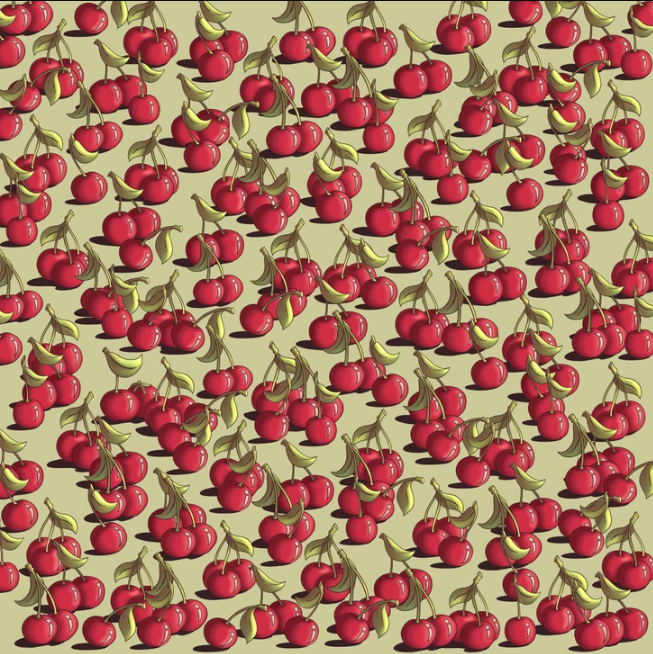
\includegraphics[width=\linewidth]{zkpimg.png}
\end{minipage}
\hfill
\begin{minipage}{0.48\textwidth}
    \centering
    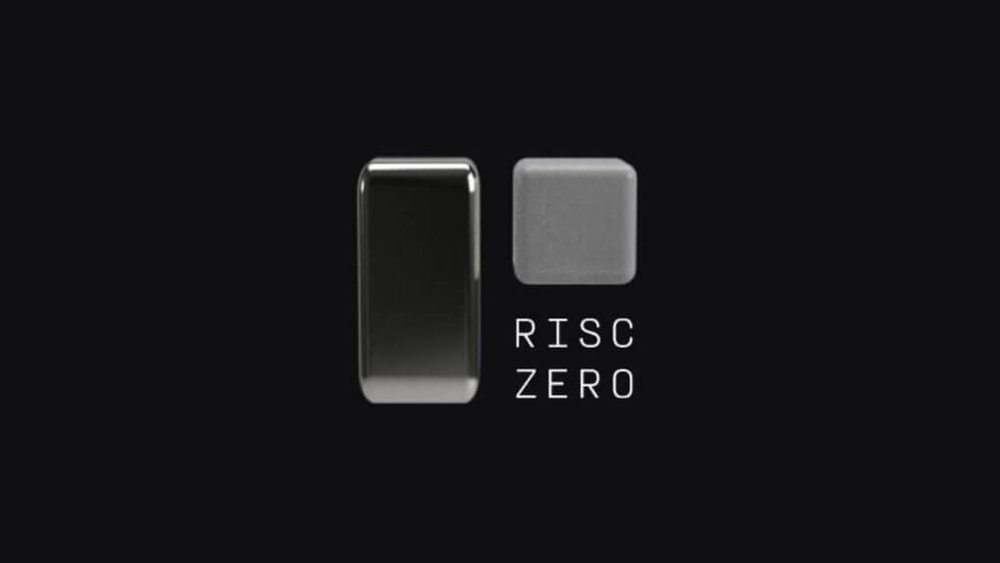
\includegraphics[width=\linewidth]{risczero.jpg}
\end{minipage}
\end{frame}

\section{Travaux effectués}

\begin{frame}
\frametitle{Conversion des flottants vers des entiers}

\begin{center}
\begin{tikzpicture}[
    box/.style = {rectangle, draw, rounded corners, minimum height=1cm, minimum width=3.5cm, align=center},
    arrow/.style = {->, thick},
    cycle/.style = {font=\small}
]

% Integer path
\node<1-> [box, fill=green!20] (intop) {Opération entière};
\node<2-> [box, fill=green!10, below=of intop] (intcycle) {1-2 cycles};
\draw<2-> [arrow] (intop) -- (intcycle);

% Float path
\node<1-> [box, fill=red!20, right=4cm of intop] (floatop) {Opération flottante};
\node<3-> [box, fill=red!10, below=of floatop] (floatsim) {Émulée en logiciel};
\node<4-> [box, fill=red!10, below=of floatsim] (floatcycle) {60-140 cycles};

\draw<3-> [arrow] (floatop) -- (floatsim);
\draw<4-> [arrow] (floatsim) -- (floatcycle);

% Comparison arrow
\draw<5-> [thick, dashed, <->] (intcycle.east) -- node[cycle, above=0.5cm, align=center] {30-100× \\ plus coûteux} (floatcycle.west);

% Labels
\node<1-> [font=\bfseries, above=0.5cm of intop] {Entiers};
\node<1-> [font=\bfseries, above=0.5cm of floatop] {Flottants};

\end{tikzpicture}
\end{center}
\end{frame}

\begin{frame}{Structures de hachage : HashMap et HashSet}

\begin{minipage}{0.6\textwidth}
\visible<1-> {
\textbf{HashMap}\\[0.3em]
\begin{tikzpicture}[
  scale=0.85, transform shape,
  node distance=0.8cm,
  box/.style={rectangle, draw, minimum width=3cm, minimum height=1cm, align=center},
  arrow/.style={->, thick}
]
\node[box] (key) {Clé};
\node[box, right=of key] (hash) {Calcul du hash};
\node[box, right=of hash] (bucket) {Emplacement};
\node[box, below=of bucket] (value) {Valeur};
\draw[arrow] (key) -- (hash);
\draw[arrow] (hash) -- (bucket);
\draw[arrow] (bucket) -- (value);
\end{tikzpicture}
}

\vspace{1em}
\visible<2->{
\textbf{HashSet}\\[0.3em]
\begin{tikzpicture}[
  scale=0.85, transform shape,
  node distance=1.5cm,
  circleNode/.style={circle, draw, minimum size=1.2cm, align=center},
  box/.style={rectangle, draw, minimum width=2.5cm, minimum height=1cm, align=center},
  arrow/.style={->, thick}
]
\node[circleNode] (elem) {Élément};
\node[box,fill=white, right=of elem] (hash) {Calcul du hash};
\node[box,fill=white, right=of hash] (bucket) {Emplacement};
\draw[arrow] (elem) -- (hash);
\draw[arrow] (hash) -- (bucket);
\end{tikzpicture}
}
\end{minipage}
\begin{minipage}{0.3\textwidth}
\visible<3->{
\begin{itemize}
  \item \textbf{HashMap} associe des clés à des valeurs.
  \item \textbf{HashSet} stocke uniquement les valeurs.
  \item Tous deux utilisent une fonction de hachage.
\end{itemize}
}
\end{minipage}

\end{frame}

% ----- Slide 2 -----
\begin{frame}{Structures arborescentes : BTreeMap et BTreeSet}

\begin{minipage}{0.4\textwidth}
\visible<1->{
\textbf{BTreeMap}\\[0.3em]
\begin{tikzpicture}[
  level distance=1.5cm,
  sibling distance=3cm,
  every node/.style={draw, rectangle, minimum width=2.5cm, minimum height=1cm, align=center},
  edge from parent/.style={draw, -latex}
]
\node {Clé 50}
  child {node {Clé 20 \\ Valeur A}}
  child {node {Clé 80 \\ Valeur B}};
\end{tikzpicture}
}
\vspace{1em}
\visible<2->{
\textbf{BTreeSet}\\[0.3em]

\begin{tikzpicture}[
  level distance=1cm,
  sibling distance=3cm,
  every node/.style={draw, circle, minimum size=1.5cm, align=center},
  edge from parent/.style={draw, -latex}
]
\node {B}
  child {node {A}}
  child {node {C}};
\end{tikzpicture}
}
\end{minipage}
\hfill
\begin{minipage}{0.5\textwidth}
\visible<3->{
\textbf{Résumé :}\\
\begin{itemize}
  \item \textbf{BTreeMap} trie les clés avec leurs valeurs.
  \item \textbf{BTreeSet} trie seulement les valeurs.
  \item Recherche et insertion par comparaison.
\end{itemize}
}
\end{minipage}

\end{frame}

\begin{frame}
\frametitle{Réduction du nombre de variables}
\begin{center}
\begin{tikzpicture}[
  scale=0.8, transform shape,
  node distance=1cm and 3cm,
  process/.style={rectangle, draw=black, rounded corners, minimum width=4.8cm, minimum height=1cm, align=center},
  comment/.style={rectangle, draw=gray, fill=gray!10, rounded corners, minimum width=5cm, align=left, font=\small},
  arrow/.style={-{Latex}, thick}
]

% Version verbeuse
\node<1->[draw=none] (before) {\textbf{Code non optimisé}};
\node<2->[process, below=of before] (v1) {let a = x + 1};
\node<3->[process, below=of v1] (v2) {let b = a * 2};
\node<4->[process, below=of v2] (v3) {let c = b - 3};
\node<5->[process, below=of v3] (vres) {Résultat final = c};

\draw<3->[arrow] (v1) -- (v2);
\draw<4->[arrow] (v2) -- (v3);
\draw<5->[arrow] (v3) -- (vres);

% Version optimisée
\node<1->[draw=none, right=4cm of before] (after) {\textbf{Code optimisé}};
\node<6->[process, below=of after] (opt1) {let res = ((x + 1) * 2) - 3};
\node<7->[process, below=of opt1] (opt2) {Résultat final = res};
\end{tikzpicture}
\end{center}
\end{frame}

\begin{frame}
\frametitle{Mémoïsation}

\begin{center}
\begin{tikzpicture}[scale=0.7, transform shape,
  node distance=1cm and 2.8cm,
  process/.style={rectangle, draw=black, rounded corners, minimum width=3cm, minimum height=1cm, align=center},
  storage/.style={rectangle, draw=blue, minimum width=2.5cm, minimum height=0.8cm, fill=blue!10},
  arrow/.style={-{Latex}, thick}
]

\visible<1->{
\node[draw=none] (before) {\textbf{Avant}};

\node[process, align=center, below=of before] (naive_start) {Calculer le burst\\ de la classe $c$};
\node[process, below=of naive_start] (naive_sum) {Recalculer $\sum_{c'>c} b^c_n$};
\node[process, below=of naive_sum] (naive_compute) {Suite des calculs ...};

\draw[arrow] (naive_start) -- (naive_sum);
\draw[arrow] (naive_sum) -- (naive_compute);

}

\visible<2->{
\node[draw=none, right=4cm of before] (after) {\textbf{Après}};

\node[process, align=center, below=of after] (opt_start) {Calculer le burst\\ de la classe $c$};
\node[storage, below=of opt_start] (opt_compute) {Stocker résultat pour la classe $c$};
\node[storage, below=of opt_compute] (opt_reuse) {Réutiliser $\sum_{c'>c} b^c_n$};
\node[process, below=of opt_reuse] (opt_store) {Suite des calculs ...};

\draw[arrow] (opt_start) -- (opt_compute);
\draw[arrow] (opt_compute) -- (opt_reuse);
\draw[arrow] (opt_reuse) -- (opt_store);
}

\end{tikzpicture}
\end{center}

\end{frame}
\section{Évaluation des performances}

\begin{frame}
  \frametitle{Graphe de l'évolution du nombre de cycles (nombre de contrats fixe)}
  \begin{center}
    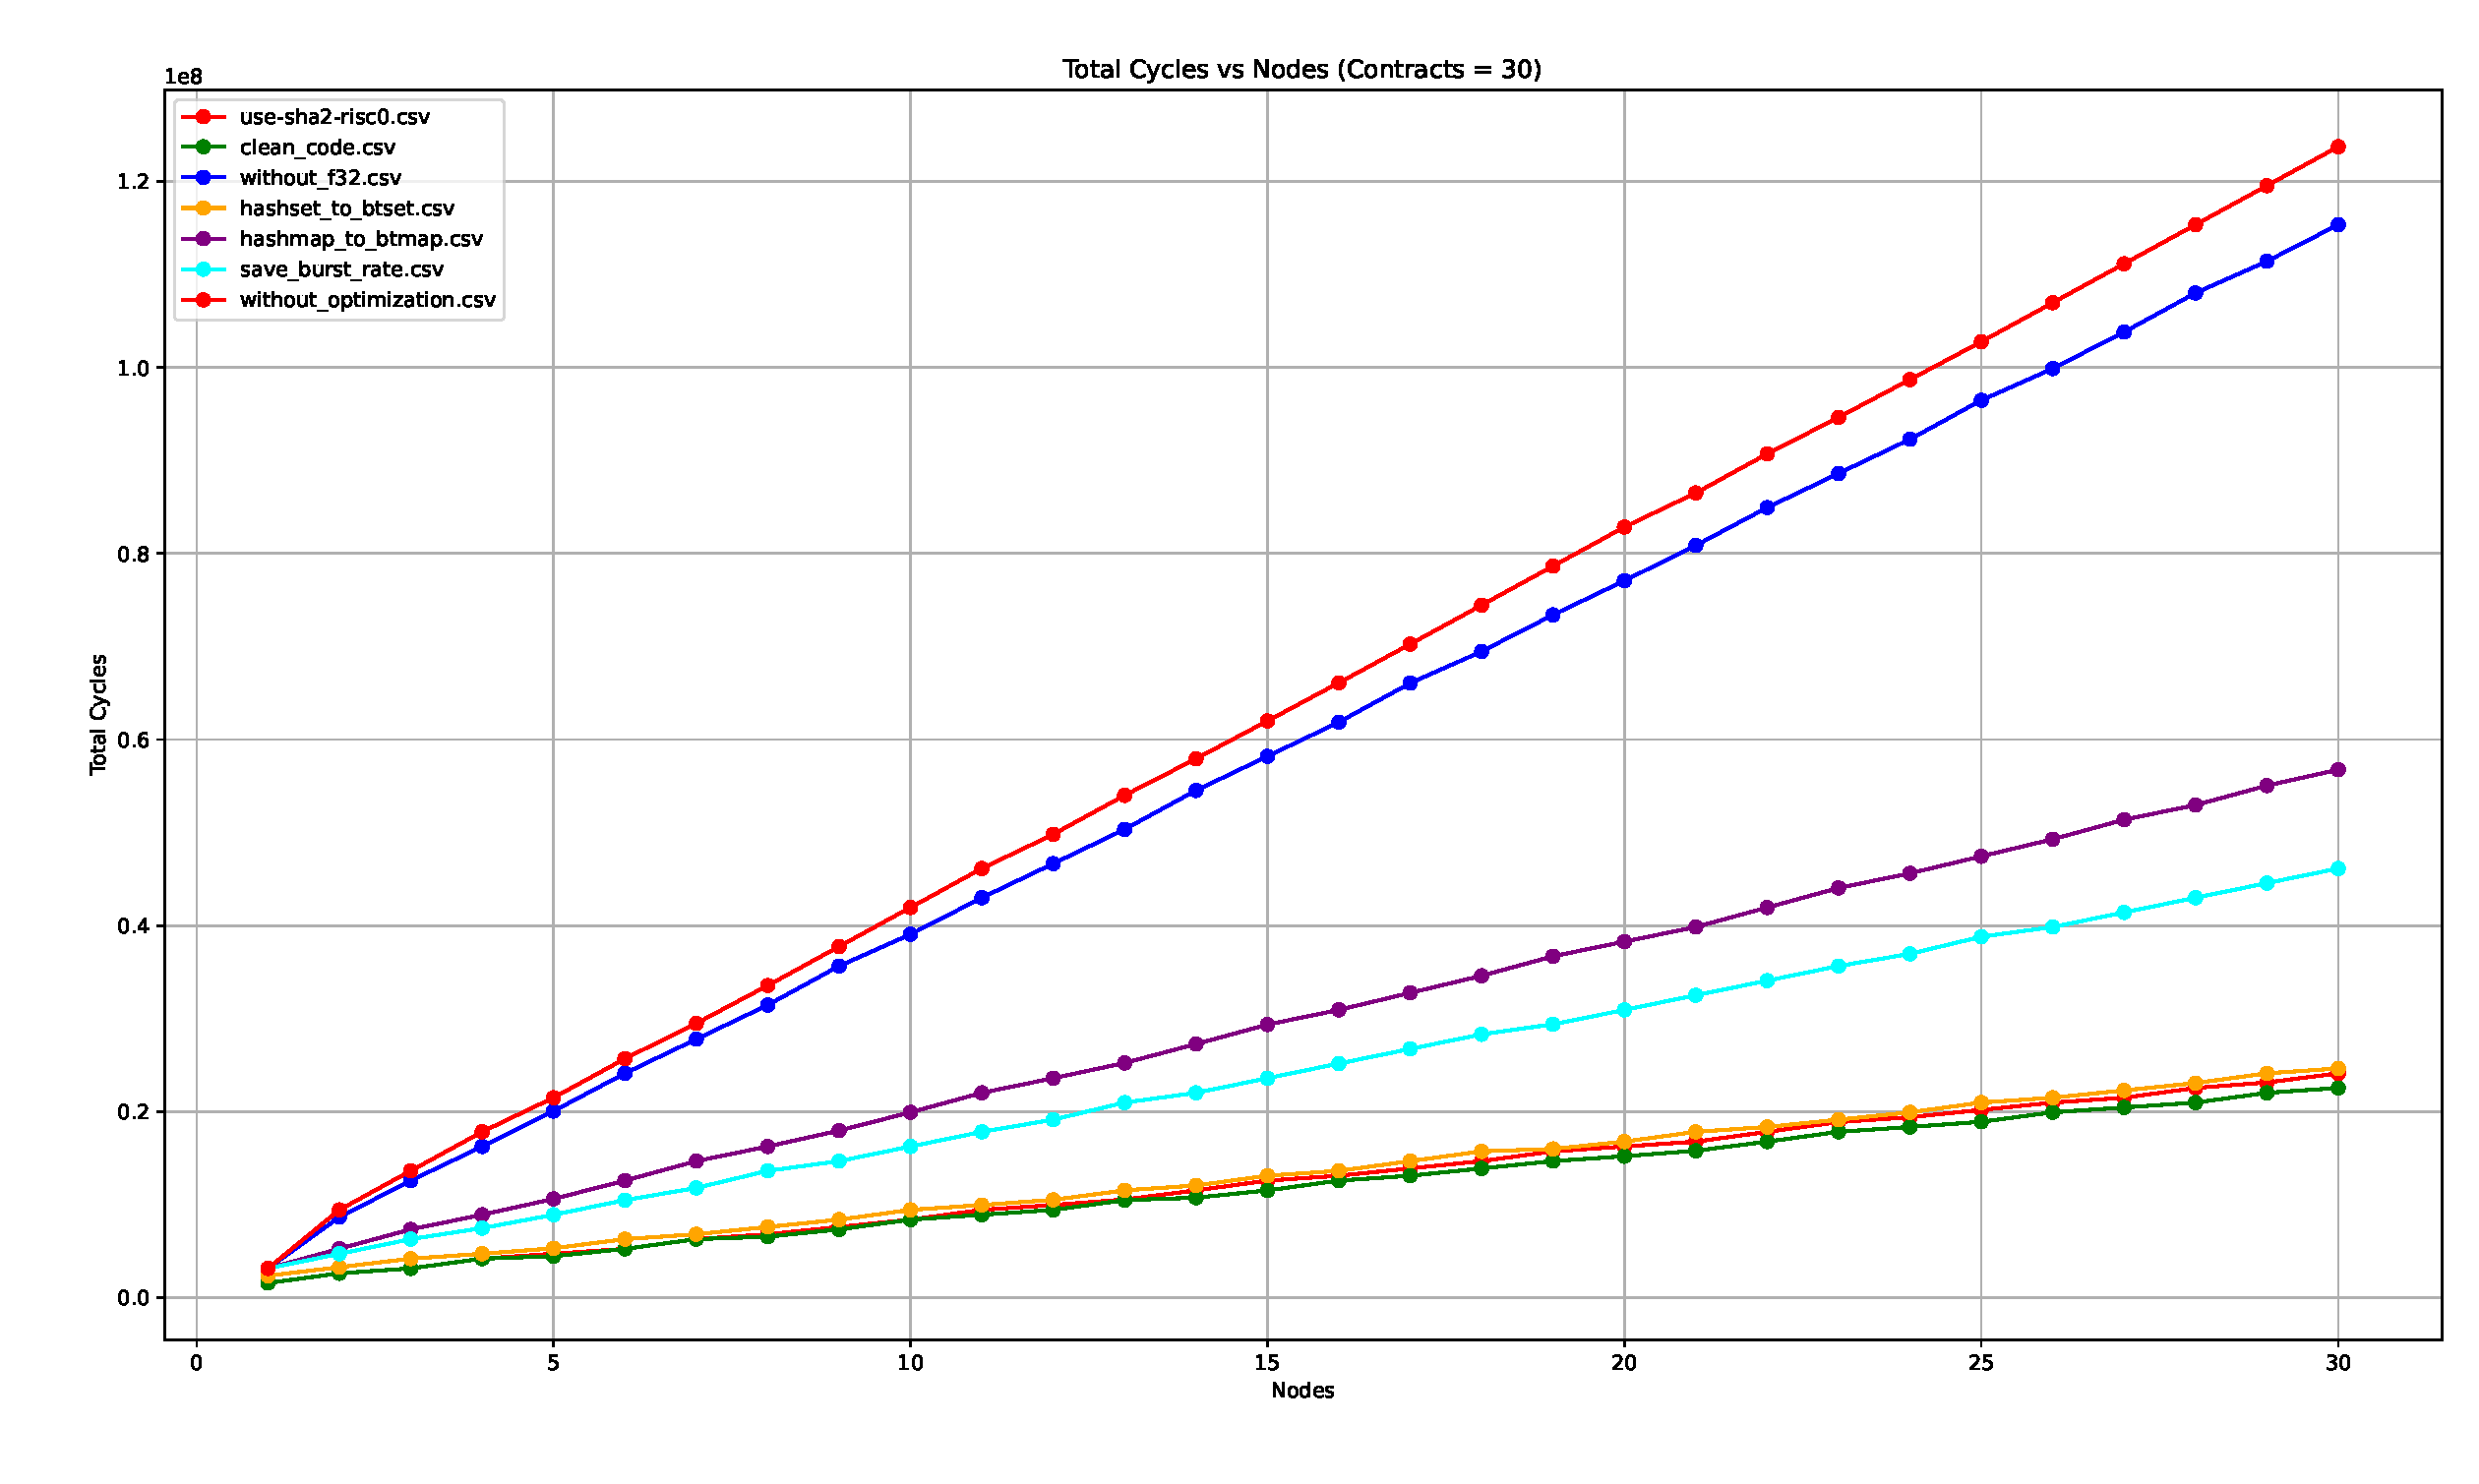
\includegraphics[scale=0.25]{benchmark_contracts.pdf}
  \end{center}
\end{frame}

\begin{frame}
  \frametitle{Graphe de l'évolution du nombre de cycles (nombre de noeuds fixe)}
  \begin{center}
    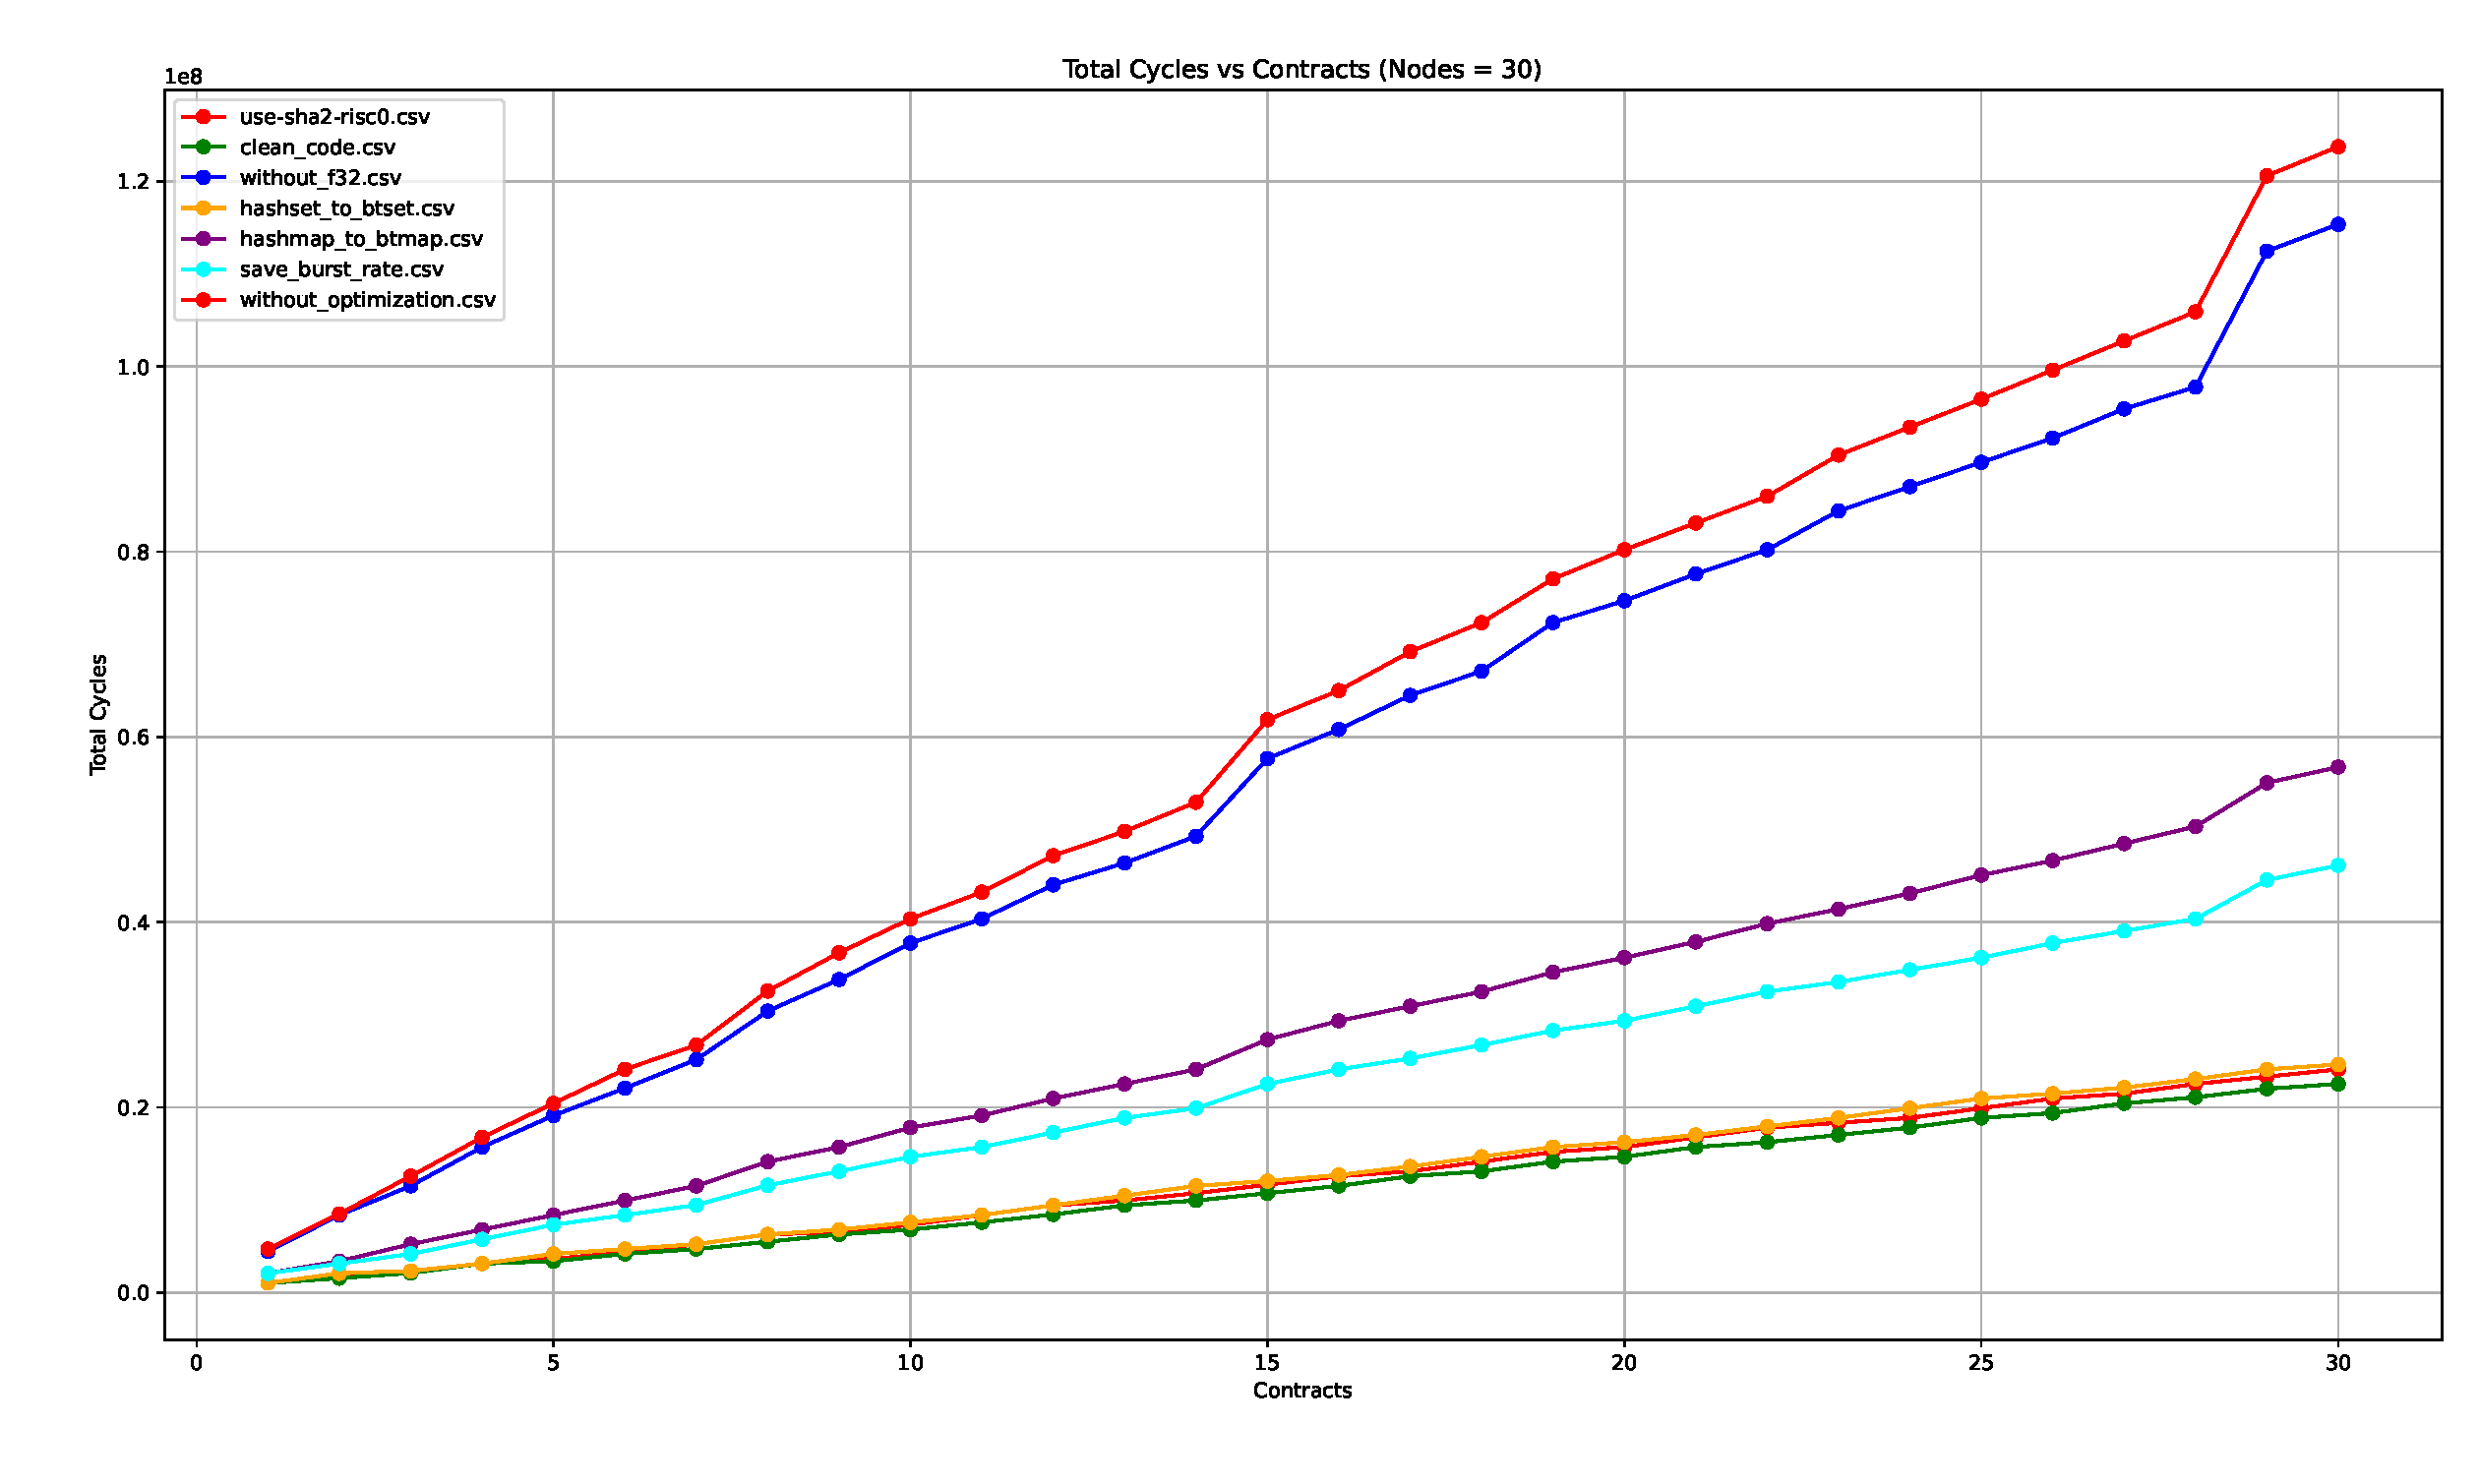
\includegraphics[scale=0.25]{benchmark_nodes.pdf}
  \end{center}
\end{frame}

\begin{frame}
  \frametitle{Tableau de synthèse}
  \begin{center}
    \begin{table}[h!]
    \centering
    \begin{tabular}{|l|r|r|r|}
    \hline
    \textbf{Optimisation} & \textbf{Cycles moyens} & \textbf{Accélération} & \textbf{Réduction (\%)} \\
    \hline
    without\_optimization.csv & 31941281.56 & 1.00x & 0.00\% \\
    without\_f32.csv       & 29764448.71 & 1.07x & 6.82\%  \\
    hashmap\_to\_btmap.csv & 14783811.13 & 2.16x & 53.72\% \\
    save\_burst\_rate.csv  & 12123104.14 & 2.63x & 62.05\% \\
    hashset\_to\_btset.csv &  6886004.05 & 4.64x & 78.44\% \\
    use\_sha2\_risc0.csv   &  6505704.11 & 4.91x & 79.63\% \\
    clean\_code.csv        &  6158727.40 & 5.19x & 80.72\% \\
    \hline
    \end{tabular}
    \end{table}
  \end{center}
\end{frame}

\section{Conclusion}
\begin{frame}[plain]
    \frametitle{Conclusion}
    \centering
    {\Huge{Merci pour votre écoute}}
\end{frame}

\section*{Bonus}
\begin{frame}
\frametitle{Algorithme TFA (vulgarisé)}
  \tikzstyle{startstop} = [rectangle, rounded corners, minimum width=3cm, minimum height=1cm,text centered, draw=black, fill=blue!20]
\tikzstyle{process} = [rectangle, minimum width=3.5cm, minimum height=1cm, text centered, draw=black, fill=orange!30]
\tikzstyle{arrow} = [thick, ->, >=Stealth]


\begin{center}
\begin{tikzpicture}[node distance=1.5cm, scale=0.9, transform shape]

% Nodes
\node<1-> (start) [startstop, align=center] {Définir le réseau et les flux \\
\footnotesize{(topologie, priorités, débit, burst)}};

\node<2-> (prio) [process, below of=start, align=center] {Analyser les priorités \\
\footnotesize{les flux les plus prioritaires sont traités en premier}};

\node<3-> (impact) [process, below of=prio, align=center] {Évaluer l’impact des flux prioritaires \\
\footnotesize{sur les flux moins prioritaires à chaque nœud}};

\node<4-> (delays) [process, below of=impact, align=center] {Déterminer le pire temps de traversée \\
\footnotesize{(latence maximale par flux)}};

\node<5-> (result) [startstop, below of=delays, align=center] {Fournir une borne supérieure \\
\footnotesize{pour la latence de chaque flux}};

% Arrows
\draw<2-> [arrow] (start) -- (prio);
\draw<3-> [arrow] (prio) -- (impact);
\draw<4-> [arrow] (impact) -- (delays);
\draw<5-> [arrow] (delays) -- (result);

\end{tikzpicture}
\end{center}
\end{frame}

\begin{frame}
\frametitle{Utilité des preuves}

\tikzstyle{startstop} = [rectangle, rounded corners, minimum width=3.5cm, minimum height=1cm, text centered, draw=black, fill=blue!20]
\tikzstyle{process} = [rectangle, minimum width=4.5cm, minimum height=1cm, text centered, draw=black, fill=orange!30]
\tikzstyle{external} = [rectangle, minimum width=4cm, minimum height=1cm, text centered, draw=black, fill=green!20]
\tikzstyle{arrow} = [thick,->,>=Stealth]

\begin{center}
\begin{tikzpicture}[node distance=1.6cm, scale=0.85, transform shape]

% Nodes
\node<1-> (exec) [process, align=center] {Exécution de TFA \\
\footnotesize{calcul des bornes de latence}};
\node<2-> (zkp) [process, below of=exec, align=center] {Génération de la preuve ZKP \\
\footnotesize{preuve que le calcul a été fait de manière honnête}};
\node<3-> (publish) [process, below of=zkp, align=center] {Publication sur la blockchain \\
\footnotesize{preuve accessible par tout le monde}};
\node<4-> (verify) [external, below of=publish, align=center] {Vérification par un contrat intelligent \\
\footnotesize{preuve validée automatiquement}};
\node<5-> (trust) [startstop, below of=verify, align=center] {Confiance garantie};

% Arrows
\draw<2-> [arrow] (exec) -- (zkp);
\draw<3-> [arrow] (zkp) -- (publish);
\draw<4-> [arrow] (publish) -- (verify);
\draw<5-> [arrow] (verify) -- (trust);

\end{tikzpicture}
\end{center}
\end{frame}

\begin{frame}
\begin{columns}
  % Left column: Steps of the algorithm
  \column{0.5\textwidth}
  \textbf{Principe.} L'algorithme parcourt les priorités dans l'ordre décroissant, puis chaque nœud du réseau. À
chaque étape, il :

  \begin{itemize}
    \item<2-> Calcule le \textbf{débit restant} au nœud.
    \item<3-> Calcule la \textbf{latence de service}.
    \item<4-> Calcule le \textbf{débit et le burst}.
    \item<5-> Calcule la \textbf{borne de latence}
    \item<6-> Propage le \textbf{burst} aux nœuds suivants.
  \end{itemize}

  % Right column: Show diagram only on slide 2
  \column{0.5\textwidth}
  \only<2>{
    \begin{tikzpicture}[scale=1.1, every node/.style={font=\small}]
      % Draw node (rectangle)
      \draw[thick] (0,0) rectangle (3,2);
      \node at (1.5,1) {\textbf{$R_n$}};
      \node at (1.5,2.3) {Nœud $n$};

      % Incoming red flows (centered, horizontal)
      \draw[->, thick, red] (-2,1.6) -- (0,1.6);
      \node at (-2.2,1.6) {$r^7_n$};

      \draw[->, thick, red] (-2,1.2) -- (0,1.2);
      \node at (-2.2,1.2) {$r^6_n$};

      \draw[->, thick, red] (-2,0.8) -- (0,0.8);
      \node at (-2.2,0.8) {$r^5_n$};

      % Bracket grouping incoming flows
      \draw[decorate,decoration={brace,amplitude=6pt},xshift=-3pt] 
        (-2,1.7) -- (-2,0.7) node[midway, left=5pt] {};

      % Remaining capacity formula
      \node at (1.5,-0.5) {\textbf{Débit restant} pour $c=4$ :};
      \node at (1.5,-1.0) {$R^c_n = R_n - \sum_{c'>c} r^{c'}_n$};
    \end{tikzpicture}
  }
  
  \only<3>{
    \begin{tikzpicture}[scale=1.1, every node/.style={font=\small}]
    % Node block
    \draw[thick] (0,0) rectangle (3,2);
    \node at (1.5,1) {\textbf{$T_n$}};
    \node at (1.5,2.3) {Nœud $n$};

    % Incoming higher-priority flows (red)
    \draw[->, thick, red] (-2,1.6) -- (0,1.6);
    \node at (-2.4,1.6) {$b^{7}_n$};

    \draw[->, thick, red] (-2,1.2) -- (0,1.2);
    \node at (-2.4,1.2) {$b^{6}_n$};

    \draw[->, thick, red] (-2,0.8) -- (0,0.8);
    \node at (-2.4,0.8) {$b^{5}_n$};

    % Bracket grouping bursts
    \draw[decorate,decoration={brace,amplitude=6pt},xshift=-3pt] 
      (-2,1.7) -- (-2,0.7);

    % Max packet size (lower priority)
    \node at (1.5,3) {$\displaystyle \frac{l_{\max}^{\leq c}}{R_n}$};

    % Output formulas
    \node at (1.5,-0.5) {\textbf{Latence de service} pour $c=4$ :};
    \node at (1.5,-1.0) {
      $T_n^c = T_n + \sum\limits_{c' > c} \frac{b^{c'}_n}{R_n^c} + \frac{l_{\max}^{\leq c}}{R_n}$
    };
    \end{tikzpicture}
  }

  \only<4>{
    \begin{tikzpicture}[scale=1.1, every node/.style={font=\small}]
      % Node block
      \draw[thick] (0,0) rectangle (3,2);
      \node at (1.5,2.3) {Nœud $n$};
    
      % Incoming flows
      \draw[->, thick, blue] (-1.7,1.6) -- (0,1.6);
      \node at (-2.2,1.6) {$r_{f_1}, b_{f_1}$};
    
      \draw[->, thick, blue] (-1.7,1.2) -- (0,1.2);
      \node at (-2.2,1.2) {$r_{f_2}, b_{f_2}$};
    
      \draw[->, thick, blue] (-1.7,0.8) -- (0,0.8);
      \node at (-2.2,0.8) {$r_{f_3}, b_{f_3}$};
    
      % Bracket
      \draw[decorate,decoration={brace,amplitude=6pt},xshift=-3pt]
        (-1.7,1.7) -- (-1.7,0.7);
    
      % Output formulas
      \node at (1.5,-0.5) {\textbf{Débit et burst} pour $c$ :};
      \node at (1.5,-1.0) {
        $r^c_n = \sum\limits_{f \in c} r_f \quad\quad b^c_n = \sum\limits_{f \in c} b_f$
      };
    \end{tikzpicture}
  }

  \only<5>{
    \begin{tikzpicture}[scale=1.1, every node/.style={font=\small}]
      % Node block
      \draw[thick] (0,0) rectangle (3,2);
      \node at (1.5,1) {\textbf{Nœud $n$}};
      \node at (1.5,2.3) {Classe $c$};

      % Inputs
      \draw[->, thick, blue] (-2,1.6) -- (0,1.6);
      \node at (-2.5,1.6) {$T_n^c$};

      \draw[->, thick, blue] (-2,1.2) -- (0,1.2);
      \node at (-2.5,1.2) {$b_n^c$};

      \draw[->, thick, blue] (-2,0.8) -- (0,0.8);
      \node at (-2.5,0.8) {$R_n^c$};

      % Bracket
      \draw[decorate,decoration={brace,amplitude=6pt},xshift=-3pt]
        (-2,1.7) -- (-2,0.7);

      % Output
      \node at (1.5,-0.5) {\textbf{Borne de latence pour $c$ :}};
      \node at (1.5,-1.0) {
        $D_n^c = T_n^c + \dfrac{b_n^c}{R_n^c}$
      };
    \end{tikzpicture}

  }

  \only<6>{
    \begin{tikzpicture}[scale=0.9, every node/.style={font=\small}]
    % Node blocks
    \draw[thick] (0,0) rectangle (3,2);
    \node at (1.5,1) {\textbf{Nœud $n$}};
    \node at (1.5,2.3) {Classe $c$};

    \draw[thick] (5,0) rectangle (8,2);
    \node at (6.5,1) {\textbf{Nœud $n+1$}};
    \node at (6.5,2.3) {Classe $c$};

    % Flow arrow
    \draw[->, thick, blue] (3,1) -- (5,1);
    \node at (4,1.4) {$f$};

    % Flow label (below)
    \node at (4,-0.3) {$b^{n+1}_f = b^n_f + r_f \cdot D^c_n$};

    \end{tikzpicture}

  }

\end{columns}
\end{frame}



\end{document}
